\section{Hinterfragen der Ethischen Korrektheit}
    In dieser Arbeit wurde neben dem Theoretischen Hintergrund [siehe \ref{sec:theorie}] auch auf die Praktische Anwendung in realen Systemen wie Smartphones [siehe \ref{subsec:FaceID_TrustedFace}] oder sogar in ganzen Ländern [siehe \ref{China:Massenueberwachung}] eingegangen. In dem folgendem Abschnitt wird nun die Ethische Korrektheit dieser Systeme untersucht. Hierbei wird sich vorallem auf die Seiten 312 & 313 der Quelle [\ref{book:religionsbuch_oberstufe}] bezogen.

    \subsection{Hinterfragen des Systems einer Künstlichen Intelligenz}
    \label{subsec:ethik_ki}
        Künstliche Intelligenz ist, wie man in dieser Facharbeit gesehen hat, ein sehr komplexes Themengebiet. Nicht unbedingt anders sieht es hier bei dem Hinterfragen der Ethischen Korrektheit von eben einer solchen KI.\\

        Betrachtet man zunächst die Nutzensethik so ist KI wohl mit eine der Theoretischen und Praktischen Systeme die hier den größten Zuspruch bekommen. Da sich die Nutzungsethik wirklich nur auf den Nutzen von etwas für den einzelnen oder die Gesellschaft bezieht kann man sich voll und ganz auf die positiven Seiten der Argumente konzentieren. Wie in [\ref{subsubsec:machnine_learning}] erfolgreich dargestellt wurde nützt uns KI schon in den alltäglichsten Dingen, wie z.B. eine neue Serie zum schauen finden die dem eigenen Interessengebiet entspricht. Auch ist Gesichtserkennung für die Sicherheit von Systemen sehr gut, aufgrund der Nutzung der biometrischen Daten eines Menschen, geignet wie es in [\ref{subsec:FaceID_TrustedFace} bzw. \ref{apple:face_id}] dargestellt wurde.\\

        Schaut man sich nun die weiteren Ethikformen an, fällt auf dass KI hier nicht unbedingt gut darsteht. Bei der Verantwortungsethik wird vorausgesetzt, dass auch Folgen des jeweiligen Handelns in die Entscheidung einfließen. Hierbei ist die Entscheidung ob es hier einen Ethischen Gewissenskonflikt gibt nicht einfach, da KI zwar lernfähig ist aber nur sinnvolle Entscheidungen für Situationen geben kann die sie trainiert hat. Somit stellt eine frisch programmierte KI, z.B. im Bereich des autonomen Fahrens, möglicherweise einen Ethischen Konflikt dar, da sie bestimmte Situationen einfach nicht beurteilen kann. Anders herum kann man aber argumentieren, dass eine langjährig trainierte KI diese Entscheidungen treffen kann. Hierbei ist allerdings zu beachten, dass es z.B. eine KI zum autonomen Fahren unmöglich alle möglichen Unfallszenarien durchlebt hat. Selbst wenn die KI über ein Netzwerk mit anderen Künstlichen Intelligenzen kommunizieren und lernen kann, so ist nicht zu 100\% sichergestellt, dass diese eine Entscheidung in einer kritischen Ausnahme Situation fällen kann. 
        
        Diese gleiche Situation sieht bei der Situationsethik allerdings anders aus. Hier wird nur auf die aktuelle Situation geschaut und nach dem bestmöglichen Ausgang für die KI gesucht. 

        \begin{wrapfigure}[10]{r}{0.25\textwidth}
            \centering
            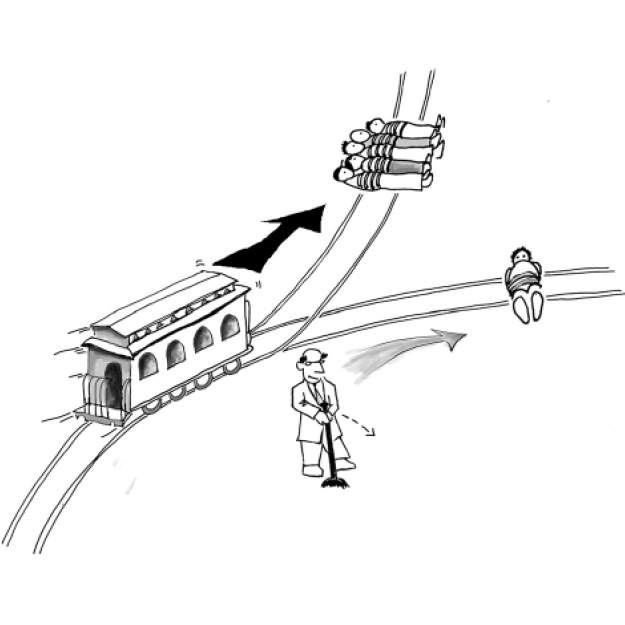
\includegraphics[width=0.25\textwidth]{resources/images/img/Gewissensfrage.jpg}
            \caption{\\[Quelle \ref{image:Gewissensfrage}]}
            \label{fig:Gewissensfrage}
        \end{wrapfigure}

        Als gutes Beispiel dient eine der Standard Gewissensfragen die normalerweise Menschen gestellt wird. Ein Zug fährt auf ein Gleis zu auf dem 4 Menschen liegen. Es gibt keine Möglichkeit ihn Aufzuhalten. Die einzige Möglichkeit diese Menschen noch zu retten ist die Weiche umzustellen. Allerdings liegt auf dem anderen Gleis auch eine Person. Die Frage: \enquote{Würdest du dir Weiche stellen?} [siehe Abbildung \ref{fig:Gewissensfrage}]\\

        Diese Frage ist für viele Menschen nicht einfach zu beantworten, da auf beiden Gleisen Menschen liegen. Eine KI würde hier relativ schnell ein Ergebnis fällen, je nachdem wie sie programmiert wurde. Höchstwahrscheinlich wird es die eine Entscheidung sein, welche den geringsten Schaden verursachen würde. Dabei würde die KI die Weiche stellen und 1 Menschenleben gegen 4 eintauschen. Auch wenn es für uns Menschen hart klingt entscheidet die KI nur Logisch.

    \subsection{Hinterfragen des Sozialpunktesystems in China}
        Im Gegensatz zu [\ref{subsec:ethik_ki}] muss bei der Ethik Hinterfragung des Sozialpunktesystems aus China keine KI die Fähigkeit zur ethischen Einschätzung haben, da es hier eher um die Frage ob es Ethisch Verantwortbar ist ein solches System für die Überwachung der Bevölkerung einzusetzen.\\
        
        Hierbei könnte die Gewissensethik durchaus als Basis der Diskussion dienen können. Allerdings würde in so einer Situation keine Antwort auf diese Frage finden, da die Gewissensethik von jedem Menschen einzeln abhängig ist.\\
        
        Vielmehr ergibt es sinn Hier auch mit der Nutzungsethik zu argumentieren. Zum einen gibt es einen großen Nutzen für Menschen mit einer hohen Punktzahl aber auch wiederum wenig Nutzen für Menschen mit einer niedrigen Punktzahl. Dieses System verpflichtet einen also fast schon dazu eine hohe Punktzahl zu besitzen, da man selbst sonst keinen Vorteil sondern sogar eher Nachteile daraus zieht.\\
        
        Andererseits ergibt sich daraus ein sehr großer Nutzen für die Gesellschaft, da der Großteil versuchen wird eine hohe Punktzahl zu erreichen. Da diese nicht durch unfaires Betrügen und Straftaten sondern dadurch gesteigert wird, dass man sich an Regeln hält, nett zu seinen Mitmenschen und sich für die Gesellschaft engagiert, hat dies eine drastische Reduzierung von Straftaten zufolge. Wobei dies auch mit der dauerhaften Überwachung in jedem Winkel zusammenhängt.
    
    \subsection{Fazit}
        Man kann Künstliche Intelligenz gut finden oder nicht. Was man aber nicht verneinen kann ist, dass KI uns in unserem Alltag schon so häufig begegnet wie es die meisten gar nicht stört sondern eher zufriedenstellt.\\
        
        Auf Basis der Nutzensethik kann man bei Künstlicher Intelligenz ganz klar von Ethischer Korrektheit reden. Das selbe gilt auch für die Situationsethik, da diese auf eine Logische neutrale Entscheidung angewiesen ist. Nur Bei der Gewissensethik kann KI, zu mindestens momentan, keine positives Ergebnis erreichen. Dies liegt ganz einfach daran, dass Computer kein Gewissen haben und wir momentan noch nicht in der Lage sind einem Computer ein Gewissen zu geben.